\setModuleTitle{Introducing The Command Line}
\setModuleAuthors{%
  Stephen Bent, Robinson Research Institute, University of Adelaide\\
  Steve Pederson, Bioinformatics Hub, University of Adelaide \mailto{stephen.pederson@adelaide.edu.au}\\
}
\setModuleContributions{%
  Dan Kortschak, Adelson Research Group, University of Adelaide \mailto{dan.kortschak@adelaide.edu.au} \\
}

%----------------------------------------------------------------------------------------
% MODULE TITLE PAGE
%----------------------------------------------------------------------------------------
% BEGIN: Module Title Page
%  * The chapter page will always appear on odd numbered page
\chapter{\moduleTitle}
\newpage

\section{Initial Goals}
\begin{enumerate}
\item Gain familiarity and confidence within the Linux command-line environment
\item Learn how to navigate directories, as well as to copy, move \& delete the files within them
\item Look up the name of a command needed to perform a specified task
\end{enumerate}


\section{Background}
Command-line tools are the mainstay of analysis of large biological data sets.
Good candidate examples for command-line analysis are:
\begin{itemize}
\item Manual inspection of fastq, bam \& sam files from NGS pipelines
\item Automating similar analyses across multiple datasets
\item Manipulations of data which are repetitive or laborious to perform manually
\item Any analysis that is different from what is available in programs with graphical interfaces (i.e. GUIs).
\item Job submission to HPC clusters
\end{itemize}  

Today we'll explore a few commands to help you gain a little familiarity with some important ones, and to enable you to find help when you're working by yourself.
We don't expect you to remember all the commands \& options from today.
The important thing is to become familiar with the basic syntax for commands, how to put them together, and where to look for help when you're unsure.


\clearpage
\section{Finding your way around}
\begin{steps}
Firstly we need to open a terminal, so either click on the terminal icon on the desktop, or go to \textit{Applications \textgreater Accessories \textgreater Terminal} on the drop-down menu at the top-left of your screen.
You will notice the text \texttt{trainee@intro-bioinf-XXX:\~{}\$} where \texttt{trainee} is the username that we have assigned to you, and \texttt{intro-bioinf-XXX} indicates which virtual machine you have been assigned to.
The tilde represents your current directory (explained later), whilst the dollar sign just indicates the end of the address \& the beginning of where you will type commands. \\
\end{steps}

\begin{note}
The terminal has a library of commands which are built into it at the time of installing the operating system, and which are part of the Bourne-again Shell, or \textit{bash}.
(Historically, it's a replacement for the earlier Bourne Shell, written by Stephen Bourne, so the name is actually a hilarious pun.)
We'll explore a few of these commands below, and the word shell will often be used interchangeably with the terminal window.
Our apologies to any purists.
If you've ever heard of the phrase \textit{shell scripts}, this refers to a series of these commands strung together into a text file which is then able to be executed as a single command.
\end{note}

\subsection{Where are we?}
\begin{steps}
Type the command \texttt{pwd} in the terminal and you will see the output \texttt{/home/trainee} appear.
\begin{lstlisting}
pwd
\end{lstlisting}
\end{steps}

\begin{information}
The command \texttt{pwd} is what we use for \underline{\textbf{p}}rinting the current (i.e. \underline{\textbf{w}}orking) \underline{\textbf{d}}irectory.
Printing in this context means to print some information to the terminal, as opposed to a physical printer.
This style of printing harks back to the days when laser printers were not commonplace.
Printing information to the terminal itself is what we refer to as printing to the \textit{standard output} or \texttt{stdout}.
\end{information}

\begin{note}
The directory path that appeared  (\texttt{/home/trainee})  is what will be referred to as your \textit{home directory} for the remainder of the workshop.
This is also the information that the tilde (\~{}) represents as a shorthand version, so whenever you see the tilde in a directory path, this is interpreted as meaning \texttt{/home/trainee}. 
The \textit{working directory} simply refers to the directory on the computer where you are currently looking, and can be thought of as being the room you are in.
We are very familiar with this concept graphically, as seen in the following image.
Instead of using a graphical view, we simply have a text-based view.\\
\end{note}

\begin{figure}[h!]
  \centering
    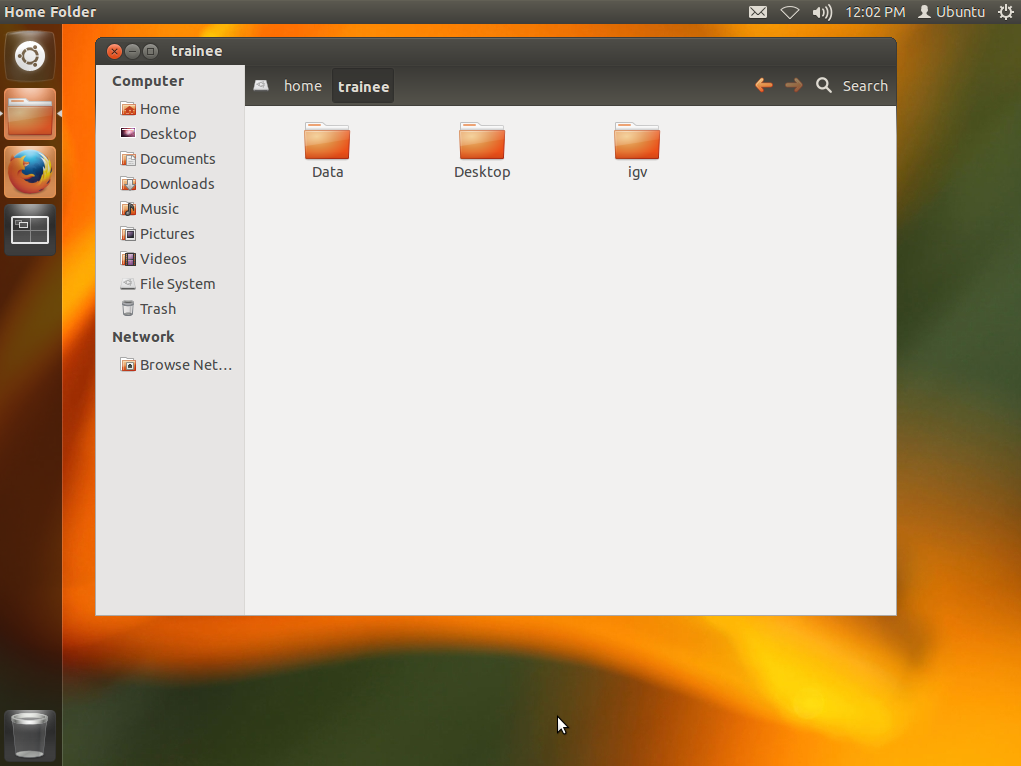
\includegraphics[width=0.9\textwidth]{home.png}
\end{figure}

\FloatBarrier
\subsection{The Linux File System}
\begin{information}
In the above command, the home directory began with a slash, i.e. \texttt{/}.
On a Linux-based system, this is considered to be the \textbf{root directory} of the file system. 
Windows users would be more familiar with seeing \texttt{C:\textbackslash} as the root of the file system, and this is a very important difference in the two directory structures.
Note also that whilst Windows uses the backslash (\textbackslash) to indicate a new directory, a Linux-based system uses the forward slash (/), or more commonly just referred to simply as ``slash'', marking another but very important difference between the two. \\
\end{information}

\begin{warning}
Although we haven't directly discovered it yet, a Linux-based file system such as Ubuntu or Mac OS-X is also \textit{case-sensitive}, whilst Windows is not.
For example, the command \texttt{PWD} is completely different to \texttt{pwd} and if \texttt{PWD} is the name of a command which has been defined in your shell, you will get completely different results than from the intended \texttt{pwd} command.

Spaces are also highly important in Linux, so take note of them where-ever they appear in the given commands.
\end{warning}

\subsubsection*{Relative vs Absolute Paths}
\begin{information}
Also note that in your output from \texttt{pwd} the resulting path started with the slash, i.e. \textbf{/}\texttt{home/trainee}.
This indicates that it is an \textbf{absolute path} as it began with the root of the file system ``/".
If the slash was missing, it would refer to a sub-directory of the current working directory, and this is what we refer to as a \textbf{relative path}.
This is an important point which will hopefully become more clear throughout the session.
\end{information}

\subsection{Changing Directories}
\begin{information}
The command \texttt{pwd} is an example of a \textit{command} that is built into the shell.
Another built-in command is \texttt{cd} which we use to \textbf{\underline{c}}hange \textbf{\underline{d}}irectory.
This changes the directory we are looking in, just like clicking our way through a directory structure in the familiar graphical style we all know well.
No matter where we are in a file system, we can move up a directory in the hierarchy by using the command 
\begin{lstlisting}
cd ..
\end{lstlisting}
The string ``\texttt{..}'' is the convention for ``\textit{one directory above}'', whilst a single dot represents the current directory. \\
\end{information}

\begin{steps}
Enter the above command and notice that the location immediately to the left of the \$ is now given as \texttt{/home}.
This is also what will be given as the output if we enter the command \texttt{pwd}.
Note that this given directory is because your personal home folder is within the folder \texttt{/home} which contains all of the home folders for all users on the computer.
If we now enter \texttt{cd ..} one more time we will be in the root directory of the file system.
Try this and print the working directory again.
As detailed earlier, the output should be the root directory given as \texttt{/}. \\
\end{steps}

We can change back to your personal home folder by entering one of either:
\begin{steps}
\begin{lstlisting}
cd /home/trainee
\end{lstlisting}
or \\
\begin{lstlisting}
cd ~ 
\end{lstlisting}
or even just \\
\begin{lstlisting}
cd
\end{lstlisting}
\end{steps}

We can also move through multiple directories in one command by separating them with the forward slash ``\texttt{/}''.
For example, we could also get to the root directory from our home directory by typing \\
\begin{lstlisting}
cd ../../ 
\end{lstlisting}

\begin{steps}
Using the above process, return to your home directory \texttt{/home/trainee}. \\
\end{steps}

\subsection{Looking at the Contents of a Directory}
\begin{steps}
There is another built-in command ``\texttt{ls}'' that we can use to \textbf{\underline{l}}i\textbf{\underline{s}}t the contents of a directory.
Enter the \texttt{ls} command as it is and it will list the contents of the current directory. \\
\begin{lstlisting}
ls 
\end{lstlisting}
\end{steps}

\begin{steps}
Alternatively, we can specify which directory we wish to view the contents of, without having to change into that directory.
We simply type the \texttt{ls} command, followed by a space, then the directory we wish to view the contents of.
To look at the contents of the root directory of the file system (i.e. \textbf{/}), we simply add that directory after the command \texttt{ls}. \\
\begin{lstlisting}
ls /
\end{lstlisting}
\end{steps}

Here you can see a whole raft of directories which contain the vital information for the computer's operating system.
Among them should be the \texttt{/home} directory which is one level above your own home directory, and where the home directories for all users are located, as mentioned earlier.\\

\begin{questions}
Try to think of two ways we could inspect the contents of the \texttt{/home} directory from your own home directory. \\
\begin{answer}
\texttt{ls /home} \\
or \\
\texttt{ls ../} \\
\end{answer}
\end{questions}

\begin{note}
Notice that there are two entries in the \texttt{/home} directory. 
One is your home directory (\texttt{/home/trainee}), whilst the other is the default home directory that came with the VM (\texttt{/home/ubuntu}) before we set up your home directory for today's workshop.
Also note that if we ever refer to this higher-level directory, we will write it as \texttt{/home}, whereas your personal home directory is always referred to without the preceding forward-slash, and will also be written in normal text font instead of the font we specifically use for code. \\
\end{note}

\subsubsection*{A Handy Hint}
\begin{information}
When working in the terminal, you can scroll through your previous commands by using the up arrow to go backward, and the down arrow to move forward.
This can be a big time saver if you've typed a long command with a simple typo, or if you have to do a series of similar commands.
\end{information}

\subsection{Going Even Deeper}
\begin{information}
So far, the commands we have used were given either without the use of any subsequent arguments, e.g. \texttt{pwd} \& \texttt{ls}, or with a specific directory as the second argument, e.g. \texttt{cd ../} \& \texttt{ls /home}.
Many commands have the additional capacity to specify different options as to how they perform, and these options are often specified between the command name, and the file being operated on.
Options are commonly a single letter prefaced with a single dash, or a word prefaced with two dashes.
The \texttt{ls} command can be given with the option \texttt{-l} specified between the command \& the directory.
This options gives the output in what is known as \textit{long listing} format. \\
\end{information}

\begin{steps}
Inspect the contents of your home directory using the long listing format. 
Please make sure you can tell the difference between the characters \texttt{l \& 1}.\\
\begin{lstlisting}
ls -l ~
\end{lstlisting}
\end{steps}

The above will give a few lines of output \& the first line should be something similar to
\begin{center}
\colorbox{black}{\texttt{\textcolor{white}{drwxr-xr-x 2 trainee trainee 4096 mmm dd hh:mm} \textcolor{light-blue}{\textbf{Desktop}}}}\\
\end{center}
where \texttt{mmm dd hh:mm} are time and date information.\\

\begin{information}
The important thing to notice is that the word \textcolor{cyan}{\texttt{Desktop}} at the end of the line will be coloured \textcolor{cyan}{\textbf{blue}}, indicating that it is a directory.
The letter `\texttt{d}' at the beginning of the initial string of codes \texttt{drwxr-xr-x} also indicates this fact.
Formally, these letters are known as flags which identify key attributes about each file or directory.
We can ignore the fine detail in the rest of these flags until this afternoon (or see the bonus section), but the values \texttt{rwx} simply refer to who is able to \textbf{\underline{r}}ead, \textbf{\underline{w}}rite or e\textbf{\underline{x}}ecute the contents of the file or directory. 
These are very helpful attributes for data security \& protection against malicious software.\\

The entries \texttt{trainee trainee} respectively refer to who is the owner of the directory (or file) \& to which group it belongs.
Again, this information won't be particularly relevant to us today, so we can ignore this until later in our programming careers.
In brief, on an Ubuntu system you could have every member of your lab group as an individual user, whilst making every member part of a group.
File access permissions can then be applied to any file based on who created it, or whether they are a member of your lab group.
Finally, the value \texttt{4096} is the size of the directory structure in bytes, whilst the date \& time refer to when the directory was created.\\

\begin{bonus}
The flags we saw at the beginning of the entries above have a clearly defined structure. 
The first entry shows the file type and for most common files, this entry will be the ``-'' seen above.
The next entries are three triplets which refer to 1) the file's owner, 2) the group they belong to \& 3) all users.
\end{bonus}

In some other entries you'll come across, the name of the file will be in \textcolor{green}{\textbf{green}}, indicating that it is a file not a directory.
There will also be a `\texttt{-}' instead of a `\texttt{d}' at the beginning of the initial string of flags. 
The remainder of the information is essentially the same as for the directories we've already seen.\\
\end{information}

\begin{advanced}
There are many more options that we could specify to give a slightly different output from the \texttt{ls} command.
Two particularly helpful ones are the options \texttt{-h} and
\texttt{-R}.
We could have specified the previous command as \\
\begin{lstlisting}
ls -l -h ~
\end{lstlisting}

This will change the file size to \textit{``human-readable''} format, whilst leaving the remainder of the output unchanged.
Try it \& you will notice that where we initially saw \texttt{4096} bytes, the size is now given as \texttt{4.0K}.
This can be particularly helpful for larger files, as most NGS files are very large indeed and seeing a file size in gigabytes will be much more informative.\\

The option \texttt{-R} tells the \texttt{ls} command to look through each directory recursively.
If we enter \\
\begin{lstlisting}
ls -l -R ~
\end{lstlisting}

the output will be given in two sections.
The first is what we have seen previously, but following that will be the contents of the directory \texttt{/home/trainee/Desktop}.
It should become immediately clear that the output from setting this option can get very large \& long depending on which directory you start from.
It's probably not a good idea to enter \texttt{ls -l -R /} as this will print out the entire contents of your file system. \\

In the case of the \texttt{ls} command we can actually specify all the above options together in the command \\
\begin{lstlisting}
ls -lhR ~
\end{lstlisting}

This can often save some time, but it is worth noting that not all programmers write their commands in such a way that this convention can be followed.
The built-in shell commands are usually fine with this, but many NGS data processing functions do not accept this convention. \\
\end{advanced}

\begin{warning}
{\Huge Don't Panic!!!}\\
It's easy for things to go wrong when working in the command-line, but if you've accidentally set something running which you need to exit or if you can't see the command prompt, there are some simple options for stopping a process \& getting you back on track.
Some options to try are: \\
\begin{tabular}{p{4cm} p{8cm}}
\centering
 & \\
 \texttt{Ctrl-c} & kill the current job.
  This is usually the first port of call when things go wrong. \\
 \texttt{Ctrl-d} & end of input. Sometimes \texttt{Ctrl-c} doesn't work but this does. \\
 \end{tabular}
Also see \texttt{man kill} or \texttt{man killall} for details on how to kill a process. \\
\end{warning}

\clearpage
\section{Exploring Commands In More Detail}

\begin{information}
In order to help us find what options are able to be specified, every command built-in to the shell has a manual, or a help page which can take some time to get familiar with.
These help pages are displayed using the pager known as \texttt{less} which essentially turns the terminal window into a text viewer so we can display text in the terminal window, but with no capacity for us to edit the text. \\
\end{information}

\begin{steps}
To display the help page for \texttt{ls} enter the command \\
\begin{lstlisting}
man ls
\end{lstlisting}
As beforehand, the space between the two is important \& in the first word we are invoking the command \texttt{man} which then looks for the \textit{manual} associated with the command \texttt{ls}.
To navigate through the manual page, we need to know a few shortcuts which are part of the \texttt{less} pager.. \\
\end{steps}

\begin{information}
Although we can navigate through the \texttt{less} pager using up \& down arrows on our keyboards, some helpful shortcuts are:\\

\begin{center}
   \begin{tabular}{p{4cm} p{8cm}}
     \hline
     \textless\texttt{enter}\textgreater & go down one line \\
     \textless\texttt{spacebar}\textgreater & go down one page (i.e. a screenful) \\
     \textbf{b} & go up (i.e. \textbf{\underline{b}}ackwards one page) \\
     \textless & go to the beginning of the document \\
     \textgreater & go to the end of the document \\
     \textbf{q} & exit (i.e. \textbf{\underline{q}}uit the page) \\
     \hline
   \end{tabular}
\end{center}
\end{information}

\begin{questions}
Look through the manual page for the \texttt{ls} command.
How could we give the directory contents in long listing format, sorted by file size? \\
\begin{answer}
\texttt{ls -l -S ~} \\
or \\
\texttt{ls -lS ~} \\
\end{answer}

Many software tools create ``\textit{hidden}" files by starting their name with a dot.
By default, these files won't be displayed using \texttt{ls}
How could we make \texttt{ls}  display these files as well as the main set of visible files.

\begin{answer}
\texttt{ls -a ~} \\
\end{answer}
\end{questions}

\begin{bonus}
We can actually find out more about the \texttt{less} pager by calling it's own \texttt{man} page.
Type the command \\
\begin{lstlisting}
man less
\end{lstlisting}
 and the complete page will appear.
This can look a little overwhelming, so try pressing \texttt{h} which will take you to a summary of the shortcut keys within \texttt{less}.
There are a lot of them, so try out a few to jump through the file. \\

A good one to experiment with would be to search for patterns within the displayed text by prefacing the pattern with a slash.
Try searching for a common word like \textit{``the''} or \textit{``to''} to see how the function behaves, then try searching for something a bit more useful, like the word \textit{``move"}. \\
\end{bonus}

\subsection{Accessing Manuals or Help Pages}
\begin{information}
As well as entering the command \texttt{man} before the name of a command you need help with, you can often just enter the name of the command with the options \texttt{-h} or \texttt{-{}-help} specified.
Note the convention of a single hyphen which indicates an individual letter will follow, or a double-hyphen which indicates that a word will follow.
Unfortunately the methods can vary a little from command to command, so if one method doesn't get you the manual, just try one of the others.\\

Sometimes it can take a little bit of looking to find something and it's important to be realise we won't break the computer or accidentally launch a nuclear bomb when we look around.
It's very much like picking up a piece of paper to see what's under it.
If you don't find something  at first, just keep looking and you'll find it eventually.\\
\end{information}

\begin{questions}
Try accessing the manual for the command \texttt{man} all three ways. 
Was there a difference in the output depending on how we asked to view the manual?\\
\begin{answer}
Yes.
Accessing the manual using \texttt{man man} displayed it a page at a time using \texttt{less}.
The other two options just printed the entire contents all at once.\\
\end{answer}


Could we access the help page for the command \texttt{ls} all three ways? \\
\begin{answer}
No.
The option \texttt{-h} gives the output in human readable format.
However, the other two methods work.\\
\end{answer}
\end{questions}

\subsection{Some Useful Commands}
\begin{steps}
So far we have explored the commands \texttt{pwd}, \texttt{cd}, \texttt{ls} \& \texttt{man} as well as the pager \texttt{less}.
Inspect the \texttt{man} pages for the commands in the following table  \& fill in the appropriate fields.
Have a look at the useful options \& try to understand what they will do if specified when invoking the command. \\

\begin{center}
\renewcommand{\arraystretch}{1.6}
\begin{tabular}{|p{2cm} | p{8.5cm} | p{4.5cm}|}
\hline
\textbf{Command} & \textbf{Description of function} & \textbf{Useful options} \\ \hline
\texttt{man} & Display on-line manual & -k (search for keywords if you don't know the command) \\ \hline
\texttt{pwd} & Print working directory, i.e show where you are & none commonly used \\ \hline
\texttt{ls} & List contents of a directory & -a, -h, -l, -S, -t, -R \\ \hline
\texttt{cd} & Change directory & (scroll down in \texttt{man builtins} to find \texttt{cd}) \\ \hline
\texttt{mv} & & -b, -f, -u \\ \hline
\texttt{cp} & & -b, -f, -u \\ \hline
\texttt{rm} & & -r (careful...) \\ \hline
\texttt{rmdir} & & \\ \hline
\texttt{mkdir} & & -p\\ \hline
\texttt{cat} & & \\ \hline
\texttt{less} & & \\ \hline
\texttt{wc} & & -l \\ \hline
\texttt{head} & & -n\# (e.g., -n100) \\ \hline
\texttt{tail} & & -n\# (e.g., -n100) \\ \hline
\texttt{echo} & &  -e\\ \hline
\texttt{cut} & & -d, -f, -s \\ \hline
\texttt{sort} & & \\ \hline
\texttt{uniq} & & \\ \hline
\end{tabular}
\end{center}
\end{steps}

\begin{bonus}
Sometimes the side effects of a command can also be useful. 
We can use \texttt{touch} to create an empty file using the command string \texttt{touch filename}.
Look at the \texttt{man} page for the command \texttt{touch} \& see if you can find this functionality described in the help page. \\
\end{bonus}

\subsection{Tab auto-complete}
\begin{steps}
A very helpful \& time-saving tool in the command line is the ability to automatically complete a command, file or directory name using the \texttt{\textless tab \textgreater} key.
Try typing 
\begin{lstlisting}
ls /home/tr <tab>
\end{lstlisting}
where \texttt{\textless tab \textgreater} represents the tab key.
\end{steps}
\begin{information}
Notice how the word \texttt{trainee} is completed automatically!
This functionality will automatically fill as far as it can until conflicting options are reached.
In this case, there was only one option so it was able to complete all the way to the end of the file path. 
This enables us to quickly enter long file paths without the risk of typos. 
Using this trick will save you an enormous amount of time trying to find why something doesn't work.
The most common error we'll see today will be mistakes in file paths caused by people not taking advantage of this trick.\\
\end{information}

\begin{steps}
Now enter
\begin{lstlisting}
ls ~/D <tab>
\end{lstlisting}
and it will look like the auto-complete is not working.
This is because there are two possibilities \& it doesn't know which you want.
Hit the tab twice and both will appear in the terminal, then choose one.
As well as directory paths, you can use this to auto-complete filenames.
\end{steps}

\begin{advanced}
This technique can be used to also find command names.
Type in \texttt{he} followed by two strike of the \texttt{\textless tab \textgreater} key and it will show you all of the commands that being with the string \texttt{he}, such as \texttt{head}, \texttt{help} or any others that may be installed on your computer.
If we'd hit the \texttt{\textless tab \textgreater} key after typing \texttt{hea}, then the command \texttt{head} would have auto-completed, although clearly this wouldn't have saved you any typing.
\end{advanced}

\section{Putting It All Together}
Now we can use some the above commands to perform something useful. \\

\begin{steps}
First, let's create a personal directory under \texttt{/home/trainee} with your first name as the directory name.
\textbf{Where you see \textit{firstname} below, use your actual firstname.}\\
\begin{lstlisting}
cd ~
mkdir firstname
\end{lstlisting}

Now we can change into this directory.
\begin{lstlisting}
cd firstname
\end{lstlisting}

Create an empty text file.
\begin{lstlisting}
touch hello.txt
\end{lstlisting}

We can read it, but it won't have anything in it yet.
\begin{lstlisting}
cat hello.txt
\end{lstlisting}

Obviously nothing was printed to your terminal in the previous line because the file is empty.
Let's write something to the file, then try reading it again.
\begin{lstlisting}
echo 'Hello' >> hello.txt
cat hello.txt
\end{lstlisting}

We can find a whole lot of information about the file.
\begin{lstlisting}
wc hello.txt
\end{lstlisting}
\end{steps}

\begin{questions}
In the previous line, what do the three numbers represent?
\begin{answer}
The lines, word \& bytes (or characters)
\end{answer}
\end{questions}

\begin{information}
When we added the word \texttt{Hello} to our file, we used the symbol $>>$ which wrote the word to the end of the file.
As the file was completely empty, this placed the word in the first line.
\end{information}

\begin{steps}
Now let's add more to the file.
\begin{lstlisting}
echo 'It's me' >> hello.txt
cat hello.txt
wc hello.txt
\end{lstlisting}
\end{steps}

\begin{note}
For most of the above commands we could have used the auto-complete feature of the bash terminal.
Did you remember this trick?
\end{note}

\begin{steps}
In the \texttt{\~{}/Documents/trainingData} directory, you will find the file \texttt{pair1.fq}
We can copy this to our newly created directory using the command \\
\begin{lstlisting}
cp ~/Documents/trainingData/pair1.fq ~/firstname/pair1.fq
\end{lstlisting}

Next we will rename the file \\
\begin{lstlisting}
mv ~/firstname/pair1.fq ~/firstname/myReads1.fq
\end{lstlisting}

We can look at the first 5 lines of the file using \\
\begin{lstlisting}
head -n5 ~/firstname/myReads1.fq
\end{lstlisting}

Or we can look at the last 10 lines of the file using \\
\begin{lstlisting}
tail -n10 ~/firstname/myReads1.fq
\end{lstlisting}

We could even page through the file using \texttt{less}.
(Remember to hit \texttt{q} to exit the pager.)\\
\begin{lstlisting}
less ~/firstname/myReads1.fq
\end{lstlisting}

We can even find how many lines there are in the file by using \\
\begin{lstlisting}
wc -l ~/firstname/myReads1.fq
\end{lstlisting}

We don't need the file anymore, so now we can delete it.
What a waste!!!
\begin{lstlisting}
rm ~/firstname/myReads1.fq
\end{lstlisting}

\end{steps}

\begin{questions}
Did we need to enter the full file path in the above commands, or could we have saved ourselves some effort by changing into the \texttt{\~{}/firstname} directory? \\
\begin{answer}
Yes, we could have changed into the \texttt{\~{}/firstname} directory \& just entered the file name. \\
\end{answer}
\end{questions}